\problemname{Dela ankor lika}
\noindent

Du är en högre makt som har fått ett viktigt uppdrag. 
Det finns $2N$ stycken kodsportsankor på ett plan, och två barn som bråkar om hur många ankor var och en ska få.

För att lösa konflikten ska du skapa en spricka i marken - en rak linje som delar planet i två delar.
Sprickan måste placeras så att exakt $N$ ankor hamnar på vardera sida.
Alla ankor har distinkta positioner med positiva heltalskoordinater.

För enkelhetens skull antar vi att sprickan kommer vara en rät linje på formen $y=kx+m$. 
Din uppgift är att hitta en spricka som delar ankorna i två lika stora delar om det går.
Skriv annars ut ”impossible”. Notera att $k$ och $m$ får vara rella tal.

\section*{Indata}
Den första raden innehåller ett heltal $N$ ($1 \leq N \leq 10^5$), där $2N$ är det totala antalet ankor.

De följande $2N$ raderna beskriver ankornas positioner.
Varje rad innehåller två heltal $x_i, y_i$ ($0 \leq x_i, y_i \leq 10^6$), koordinaterna för den $i$:te ankan.
Alla ankor har olika positioner.

\section*{Utdata}
Om det är möjligt att dela ankorna lika, skriv ut två reella tal $k$ och $b$ ($-5*10^9 \leq k, b \leq 5*10^9$) som beskriver linjen $y = kx + b$.
Svaret accepteras om det finns en linje med dina värden som delar ankorna korrekt.

Om det är omöjligt att dela ankorna lika, skriv ut ”impossible”.

\section*{Poängsättning}
Din lösning kommer att testas på en mängd testfallsgrupper.
För att få poäng för en grupp så måste du klara alla testfall i gruppen.

\noindent
\begin{tabular}{| l | l | p{12cm} |}
  \hline
  \textbf{Grupp} & \textbf{Poäng} & \textbf{Gränser} \\ \hline
  $1$    & $15$       & $N = 1$ \\ \hline
  $2$    & $15$       & $x_i = 0$ för alla ankor. \\ \hline
  $3$    & $15$       & $x_i \leq 1$ för alla ankor. \\ \hline
  $4$    & $15$       & $N = 2$ \\ \hline
  $5$    & $20$       & $N \leq 1000$ \\ \hline
  $6$    & $20$       & Inga ytterligare begränsningar. \\ \hline
\end{tabular}

\section*{Förklaring av exempelfall}
Notera att det finns fler giltiga lösningar i alla dessa fallen.

\begin{centering}
  \begin{figure}[h]
      \centering
      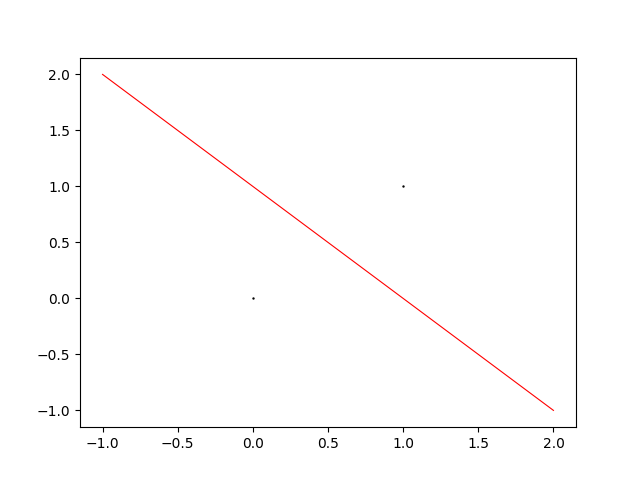
\includegraphics[width=0.3\textwidth]{sample1.png}
      \caption{Bilden föreställer första exempelfallet. Vara anka representeras av en prick, och sprickan är den röda linjen.}
      \label{fig:enter-label}
  \end{figure}
\end{centering}

\begin{centering}
  \begin{figure}[h]
      \centering
      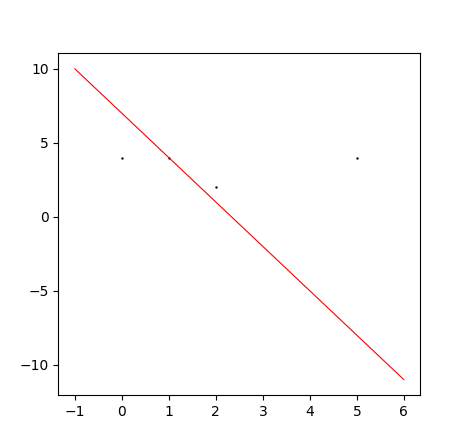
\includegraphics[width=0.3\textwidth]{sample2.png}
      \caption{Bilden föreställer andra exempelfallet. Vara anka representeras av en prick, och sprickan är den röda linjen. Det är svårt att se, men den andra punkten
      är precis ovanför linjen.}
      \label{fig:enter-label}
  \end{figure}
\end{centering}

\begin{centering}
  \begin{figure}[h]
      \centering
      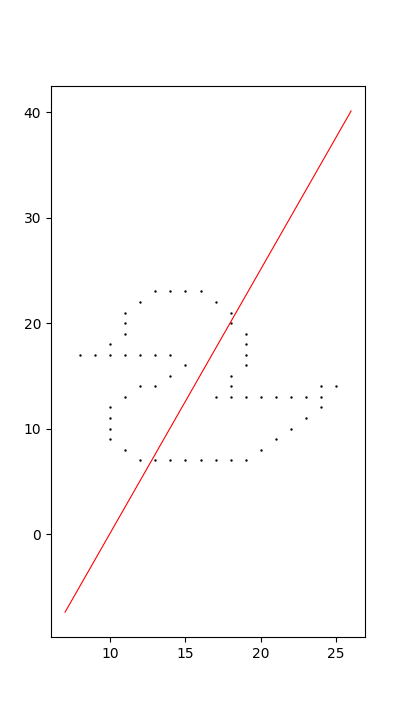
\includegraphics[width=0.3\textwidth]{sample3.png}
      \caption{Bilden föreställer tredje exempelfallet. Vara anka representeras av en prick, och sprickan är den röda linjen.}
      \label{fig:enter-label}
  \end{figure}
\end{centering}